\documentclass[pdflatex,sn-mathphys-num]{sn-jnl}

%%%% Standard Packages
\usepackage{graphicx}%
\usepackage{multirow}%
\usepackage{amsmath,amssymb,amsfonts}%
\usepackage{amsthm}%
\usepackage{mathrsfs}%
\usepackage[title]{appendix}%
\usepackage{xcolor}%
\usepackage{textcomp}%
\usepackage{manyfoot}%
\usepackage{booktabs}%
\usepackage{comment}
\usepackage{algorithm}%
\usepackage{algorithmicx}%
\usepackage{algpseudocode}%
\usepackage{listings}%
\usepackage{float}%

\newcommand{\placeholderfig}[2]{%
  \fbox{\parbox[c][#1][c]{0.92\textwidth}{\centering\sffamily\small
  [FIGURA PENDIENTE]\\[0.4em]#2}}%
}

\raggedbottom

\begin{document}

\title[]{}
\author*[1,2]{\fnm{Sergio} \sur{Morales Méndez}}\email{s.morales01@ufromail.cl}
%\orcid{0000-0001-7848-8008}
\author[3]{\fnm{Andrés I.} \sur{Ávila}}\email{andres.avila@ufrontera.cl}

\author[4,5]{\fnm{Mailyn} \sur{Moreno Espino}}\email{mailymor@ucm.es}

\author[2]{\fnm{Oscar} \sur{Valderrama Cayumán}}\email{oscar.valderrama@sernageomin.cl}


\affil[1]{\orgdiv{Programa de Doctorado en Ingeniería}, \orgname{Universidad de La Frontera}, \orgaddress{\street{Francisco Salazar 01145}, \city{Temuco}, \postcode{4811230}, \country{Chile}}}

\affil[2]{\orgdiv{Observatorio Volcanológico de los Andes del Sur (OVDAS)}, \orgname{Servicio Nacional de Geología y Minería (SERNAGEOMIN)}, \orgaddress{\street{Rudecindo Ortega 03786}, \city{Temuco}, \postcode{4780000}, \country{Chile}}}

\affil[3]{\orgdiv{Departamento de Ingeniería Matemática}, \orgname{Universidad de La Frontera}, \orgaddress{\street{Francisco Salazar 01145}, \city{Temuco}, \postcode{4811230}, \country{Chile}}}

\affil[4]{\orgdiv{Facultad de Informática}, \orgname{Universidad Complutense de Madrid}, \orgaddress{\city{Madrid}, \country{España}}}

\affil[5]{\orgdiv{Instituto de Tecnología del Conocimiento}, \orgname{Universidad Complutense de Madrid}, \orgaddress{\city{Madrid}, \country{España}}}

\abstract{}
\keywords{}
\maketitle

%%===========================================================================%%
\section{Introduction}\label{sec:intro}

\section{Data}\label{sec:data}

\subsection{Volcanic systems and monitoring network}\label{subsec:area}

The analysis uses the seismic catalog maintained by the Southern Andes
Volcanological Observatory (OVDAS), the agency responsible for permanent volcano
monitoring in southern Chile within Chile's National Geology and Mining Service
(SERNAGEOMIN) \cite{amigo_volcano_2021}. OVDAS operates dedicated local seismic
networks at the active volcanoes under surveillance and maintains continuous
event catalogs for each monitored system. The five volcanic systems were selected according to three criteria. First,
their catalogs provide sufficient event volumes to preserve class support
under the partitions defined in Section~\ref{sec:methods}. Second, their
combined catalogs include the event classes of interest, with class
availability distributed across the five systems. Third, they represent
distinct volcanic environments and therefore provide a basis for assessing
classification behavior across heterogeneous seismicity and recording
conditions.

The third criterion defines the scientific contrast within the dataset.
Villarrica is an open-conduit system with an active lava lake and
near-continuous long-period (LP) seismicity
\cite{richardson_varying_2014}. Nevados de Chill\'an has sustained an eruption
with alternating effusive and explosive phases since 2016
\cite{cardona_volcanic_2021}. Copahue exhibits persistent hydrothermal
circulation \cite{casas_single-station_2024}. Laguna del Maule has undergone a
prolonged volcano-tectonic (VT) swarm associated with inflation of its
magmatic-hydrothermal system \cite{cardona_crustal_2018}. Hudson is a heavily
glaciated stratovolcano whose catalog includes brittle-fracture, fluid-resonance,
and surface-process seismicity \cite{agurto-detzel_seismicity_2014}. Together, these systems provide contrasting volcanic settings, seismicity
rates, and catalog compositions, enabling evaluation across heterogeneous
source and recording environments.

The five systems span approximately 1100~km along the Southern Volcanic
Zone, from Laguna del Maule in the north to Hudson in the south, and each is
monitored by an independent local seismic network (Figure~\ref{fig:map}). One
vertical-component channel per volcano was selected for waveform analysis,
following the station-selection criterion of
Section~\ref{subsec:stationselection}, with all channels sampled at 100~Hz
(Table~\ref{tab:stations}). The selected waveform records reflect system-specific differences in
instrument response, source--station distance, site conditions, and event
population, and every quantity reported in this paper is accordingly
computed within a single system. The analyzed interval of a system, narrower
than the nominal 2013--2024 request at three of the five systems, is the
span over which its selected station appears as the detecting station in the
catalog (Table~\ref{tab:stations}). Laguna del Maule begins in
April 2021, shortly after station NI2Z entered operation on 30 March 2021.
Copahue ends in August 2024 and Hudson in January 2024; both catalogs continue
to December 2024 through other stations of their local networks, but the
selected station stops appearing as the detecting station on those dates.
Hudson also begins in March 2013 rather than January, because no station record
covering the analysis window of Section~\ref{subsec:conditioning} is
recoverable for its earlier entries. Nevados de Chill\'an and Villarrica span
the full January 2013--December 2024 interval.

\begin{table}[h]
\caption{Station selected at each volcanic system and the interval it defines. The analyzed interval is the span actually covered by the events of Table~\ref{tab:counts}, not the nominal 2013--2024 request.}\label{tab:stations}
\begin{tabular}{@{}lccc@{}}
\toprule
Volcanic system & Station & Crater distance (km) & Analyzed interval \\
\midrule
Laguna del Maule      & NI2Z & 7.4 & 2021-04--2024-12 \\
Nevados de Chill\'an  & FREZ & 1.6 & 2013-01--2024-12 \\
Copahue               & MAHZ & 3.7 & 2013-01--2024-08 \\
Villarrica            & VN2Z & 3.1 & 2013-01--2024-12 \\
Hudson                & HUDZ & 9.3 & 2013-03--2024-01 \\
\botrule
\end{tabular}
\end{table}

\begin{figure}[H]
\centering
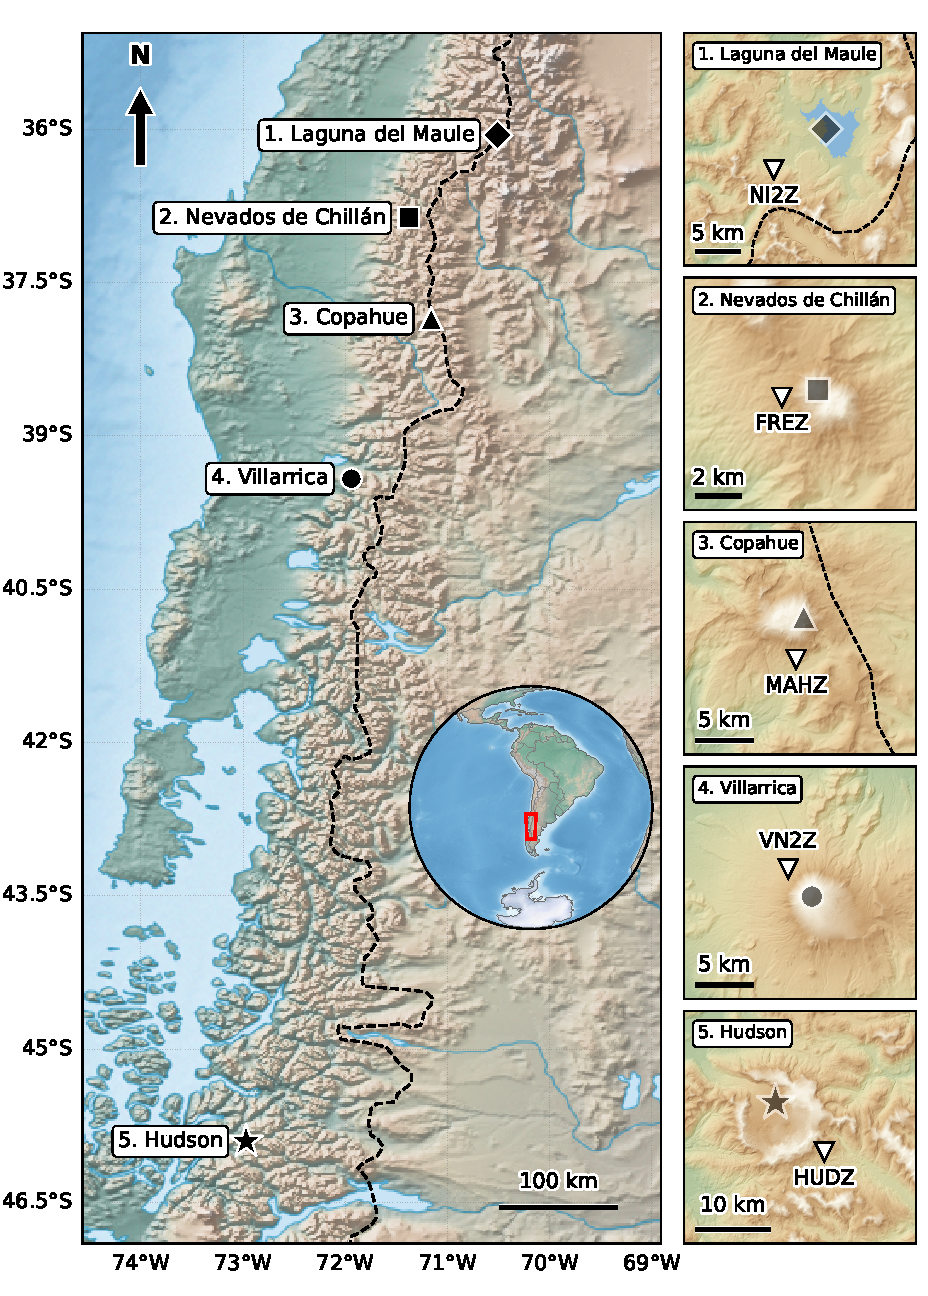
\includegraphics[width=0.94\textwidth]{fig_map.pdf}
\caption{Location of the five volcanic systems and their selected stations,
numbered 1--5 consistently across panels. Left: regional view of the Southern
Volcanic Zone, from Laguna del Maule to Hudson, with a distinct symbol per
volcano, the Chile-Argentina border dashed, and a globe inset locating the
region (red rectangle). Right: shaded-relief local views centered between each
crater (filled symbol) and its station (open triangle, labeled with the code
given in Table~\ref{tab:stations}); lakes appear in blue and the international
border is repeated where it falls within a panel. The local panels share a
common size but not a common scale, each zoomed to its own crater-station
separation, so the scale bar must be read panel by panel. Topography from
Natural Earth (regional panel and inset) and Terrarium elevation tiles (local
panels). Coordinates in WGS84.}
\label{fig:map}
\end{figure}



\subsection{Nature of the catalog}\label{subsec:catalog}

The catalog results from analyst-based operational classification. For each
event, the analyst assigns an event class, identifies a detecting station,
selects an onset or phase-pick reference, and records a duration. This
reference time corresponds to the analyst-selected arrival at the detecting
station and provides the temporal reference for waveform-window extraction.
Duration is assigned during operational labeling and is therefore treated as a
catalog attribute.

Duration separates the classes as clearly as any waveform attribute, and it
varies between systems for a single class. Taken across the systems where a
class reaches support, median analyst-assigned durations run from 8.4~s for
VT to 36.0~s for TO, with HB, VLP, LP and AV in between
(Table~\ref{tab:durations}). The same class also shifts between systems: LP
has a median duration of 11.0~s at Copahue and 29.7~s at Villarrica, and VT
of 8.0~s at Laguna del Maule and 17.9~s at Villarrica. Most cataloged events
therefore last longer than the fixed window of
Section~\ref{subsec:conditioning}, which spans 11.9\% of the analyzed
population in full; for the rest, that window covers the onset and the early
coda. Section~\ref{subsec:configuration} reports the proportion per system.

A small number of entries carry a non-positive duration, 1{,}457 events or
0.099\% of the analyzed population. They are retained as they appear in the
catalog, since duration enters no step of the pipeline: the analysis window
is defined from the onset alone (Section~\ref{subsec:conditioning}).

\begin{table}[h]
\caption{Median analyst-assigned duration in seconds, by volcanic system and
class, over the analyzed population. Only volcano-class combinations reaching
the support criterion of Section~\ref{subsec:classsupport} are shown. Each
median is taken within one system: the systems differ in station and in class
composition, so a figure spanning them would describe no population that was
recorded.}\label{tab:durations}
\begin{tabular}{@{}lrrrrrr@{}}
\toprule
Volcano & LP & VT & HB & VLP & AV & TO \\
\midrule
Laguna del Maule      & 17.4 & 8.0  & --   & --   & --   & --   \\
Nevados de Chill\'an  & 28.0 & 13.0 & --   & 20.0 & 40.0 & 36.0 \\
Copahue               & 11.0 & 8.0  & 7.0  & 22.0 & --   & --   \\
Villarrica            & 29.7 & 17.9 & --   & --   & 27.0 & --   \\
Hudson                & 21.6 & 8.4  & 25.6 & --   & 20.0 & --   \\
\botrule
\end{tabular}
\end{table}

Hypocentral solutions are available for a subset of the cataloged events.
Operational monitoring prioritizes timely event characterization, and event
classification consequently proceeds independently of a location estimate for
most entries. Event descriptions therefore rely on waveform-derived attributes,
while similarity groups are inferred from waveform resemblance rather than
from hypocentral proximity.

\subsection{Event classes and scope of the analysis}\label{subsec:classes}

The OVDAS database contains a broader set of operational codes than the subset
used in the analysis, based on classification proposed by \cite{lahr_earthquake_1994} and \cite{chouet_volcano_2003}. The retained population comprises six operational volcano-seismic classes:
LP (long-period), VT (volcano-tectonic), HB (hybrid), VLP
(very-long-period; coded LV in the database), AV (avalanche and rockfall),
and TO (tornillo). Between 2013 and 2024, these classes account for 63--97\% of
catalog entries across the five systems (Table~\ref{tab:rawcounts}).

\begin{table}[h]
\caption{Catalogued entries between 2013 and 2024 at all stations of each local
network, before the selection criteria of Section~\ref{sec:methods}.}\label{tab:rawcounts}
\begin{tabular}{@{}lrrrr@{}}
\toprule
Volcano & Catalog total & Six retained classes & TR & Other codes \\
\midrule
Laguna del Maule
& 128{,}859
& 124{,}563 (96.7\%)
& 279 (0.2\%)
& 4{,}017 (3.1\%) \\
Nevados de Chill\'an
& 520{,}873
& 329{,}928 (63.3\%)
& 92{,}185 (17.7\%)
& 98{,}760 (19.0\%) \\
Copahue
& 160{,}526
& 150{,}405 (93.7\%)
& 5{,}643 (3.5\%)
& 4{,}478 (2.8\%) \\
Villarrica
& 1{,}198{,}979
& 1{,}008{,}464 (84.1\%)
& 112{,}301 (9.4\%)
& 78{,}214 (6.5\%) \\
Hudson
& 53{,}314
& 46{,}275 (86.8\%)
& 60 (0.1\%)
& 6{,}979 (13.1\%) \\
\botrule
\end{tabular}
\end{table}

Tremor (TR) is omitted because the code represents sustained or composite
seismic radiation rather than a consistently delimited discrete event. Sustained
tremor and dense sequences of LP events may generate comparable records, and
their operational separation can therefore depend on the temporal organization
of the signal. Restricting the analysis to discrete-event classes preserves a
common unit of observation across the dataset.

Three further database codes are excluded because they do not denote waveform
classes at all. EX marks an event with an observed surface manifestation, and
MF an event accompanied by an acoustic signal. Both are observational
attributes rather than mutually exclusive categories, since either can
accompany LP, HB, or tremor seismicity, and excluding them preserves a class
axis defined exclusively by waveform type. VA marks an event below the
amplitude threshold required for assignment to any specific waveform class,
and therefore denotes an operational detection category rather than a source
or signal type.

\begin{figure}[H]
\centering
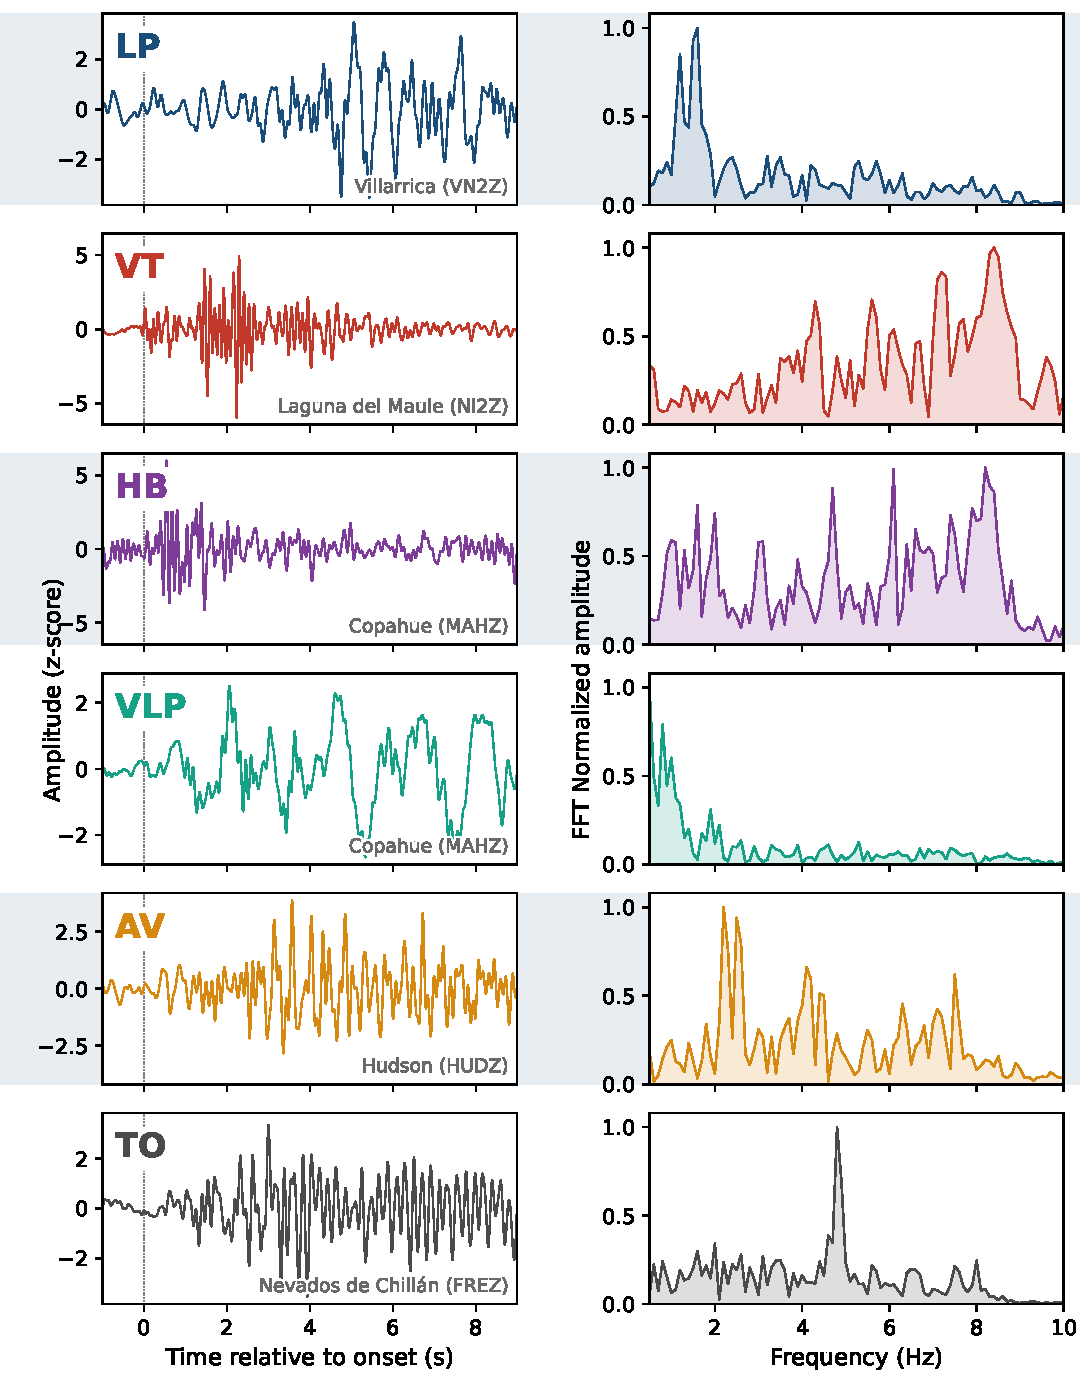
\includegraphics[width=0.92\textwidth]{fig_gallery.pdf}
\caption{Representative waveforms and amplitude spectra for each retained event
class, with one row per class (LP, VT, HB, VLP, AV, and TO). The volcano and
station of each example are indicated in the waveform panel. Left: the first
10~s from the onset, the window defined in
Section~\ref{subsec:conditioning}, shown for every class irrespective of the
analyst-assigned duration of the event. Right: amplitude spectrum of the same window,
normalized by its maximum amplitude. Both panels show the conditioned signal
window of Section~\ref{subsec:conditioning}, the record from which the
descriptors are computed.}
\label{fig:gallery}
\end{figure}

The six retained classes are assigned by analysts from waveform morphology and
spectral content and therefore represent operational signal categories rather
than direct determinations of source mechanisms
(Figure~\ref{fig:gallery}). The waveform-based descriptions below summarize
the interpretations commonly associated with these labels and are not treated
as independent measurements of source processes. LP events are characterized
by emergent onsets and narrow-band low-frequency energy, commonly associated
with resonance in fluid-filled cracks
\cite{chouet_long-period_1996}. VT events are characterized by impulsive
onsets and broadband energy extending toward higher frequencies, consistent
with signals commonly associated with brittle rock failure. HB events combine
an impulsive onset with a low-frequency coda
\cite{white_volcano-tectonic_2016}. VLP events are characterized
operationally by lower-frequency energy than LP events and may be
associated with slow fluid transport or conduit deformation
\cite{almendros_identifying_2002}. AV events are typically emergent,
broadband, and relatively long-duration surface signals
\cite{heck_localization_2019}. TO events exhibit slowly decaying,
quasi-monochromatic codas \cite{gomez_m_tornillo_1999}. The classes occupy
partially overlapping regions of waveform and spectral feature space; HB, in
particular, occupies a transitional region between LP and VT signals.



\subsection{Class composition}\label{subsec:composition}

The analyzed population results from two sequential filters applied to the
six-class catalog of Table~\ref{tab:rawcounts}, defined in
Section~\ref{subsec:conditioning}: one restricting events to the station
listed in Table~\ref{tab:stations}, the other requiring a complete analysis
window. These filters retain 73--95\% of the six-class catalog, depending on
the volcano, and yield an analyzed population of 1{,}477{,}410 events.
Section~\ref{subsec:configuration} reports the contribution of each filter
separately. The population is counted over distinct events: the catalog
repeats a small number of entries, the same event identifier at the same
time, and each is retained once. Section~\ref{subsec:configuration} reports how many
entries this affects at each system.

\begin{table}[h]
\caption{Composition of the analyzed set by volcanic system and class.}\label{tab:counts}
\begin{tabular}{@{}lrrrrrr@{}}
\toprule
Volcano & LP & VT & HB & VLP & AV & TO \\
\midrule
Laguna del Maule
& 446 & 102{,}962 & 22 & 0 & 46 & 0 \\
Nevados de Chill\'an
& 233{,}665 & 14{,}312 & 16 & 3{,}208 & 16{,}338 & 472 \\
Copahue
& 36{,}226 & 7{,}304 & 65{,}958 & 3{,}058 & 1 & 0 \\
Villarrica
& 952{,}458 & 314 & 1 & 23 & 6{,}440 & 0 \\
Hudson
& 10{,}940 & 15{,}035 & 483 & 0 & 7{,}682 & 0 \\
\botrule
\end{tabular}
\end{table}

Class composition varies strongly among volcanic systems
(Table~\ref{tab:counts}). LP represents 99.3\% of the analyzed population at
Villarrica, whereas VT represents 99.5\% at Laguna del Maule. HB is the
dominant class at Copahue, accounting for 58.6\% of its analyzed population.
Nevados de Chill\'an contains five classes with substantial support, with LP
representing 87.2\% of its analyzed population. Hudson has the most even class
distribution among the five systems: VT, LP, and AV represent 44.0\%, 32.0\%,
and 22.5\% of the analyzed population, respectively, while HB contributes
1.4\%. These system-specific proportions are consistent with contrasting seismicity
regimes and provide a basis for evaluating the sensitivity of classification
results to alternative event-partitioning strategies. Two cells of this matrix hold a single event: one HB at Villarrica and one AV
at Copahue. We report both as they appear in the catalog and treat them as
isolated cases throughout, since a class with one representative supports no
estimate of within-class variability.

\begin{figure}[H]
\centering
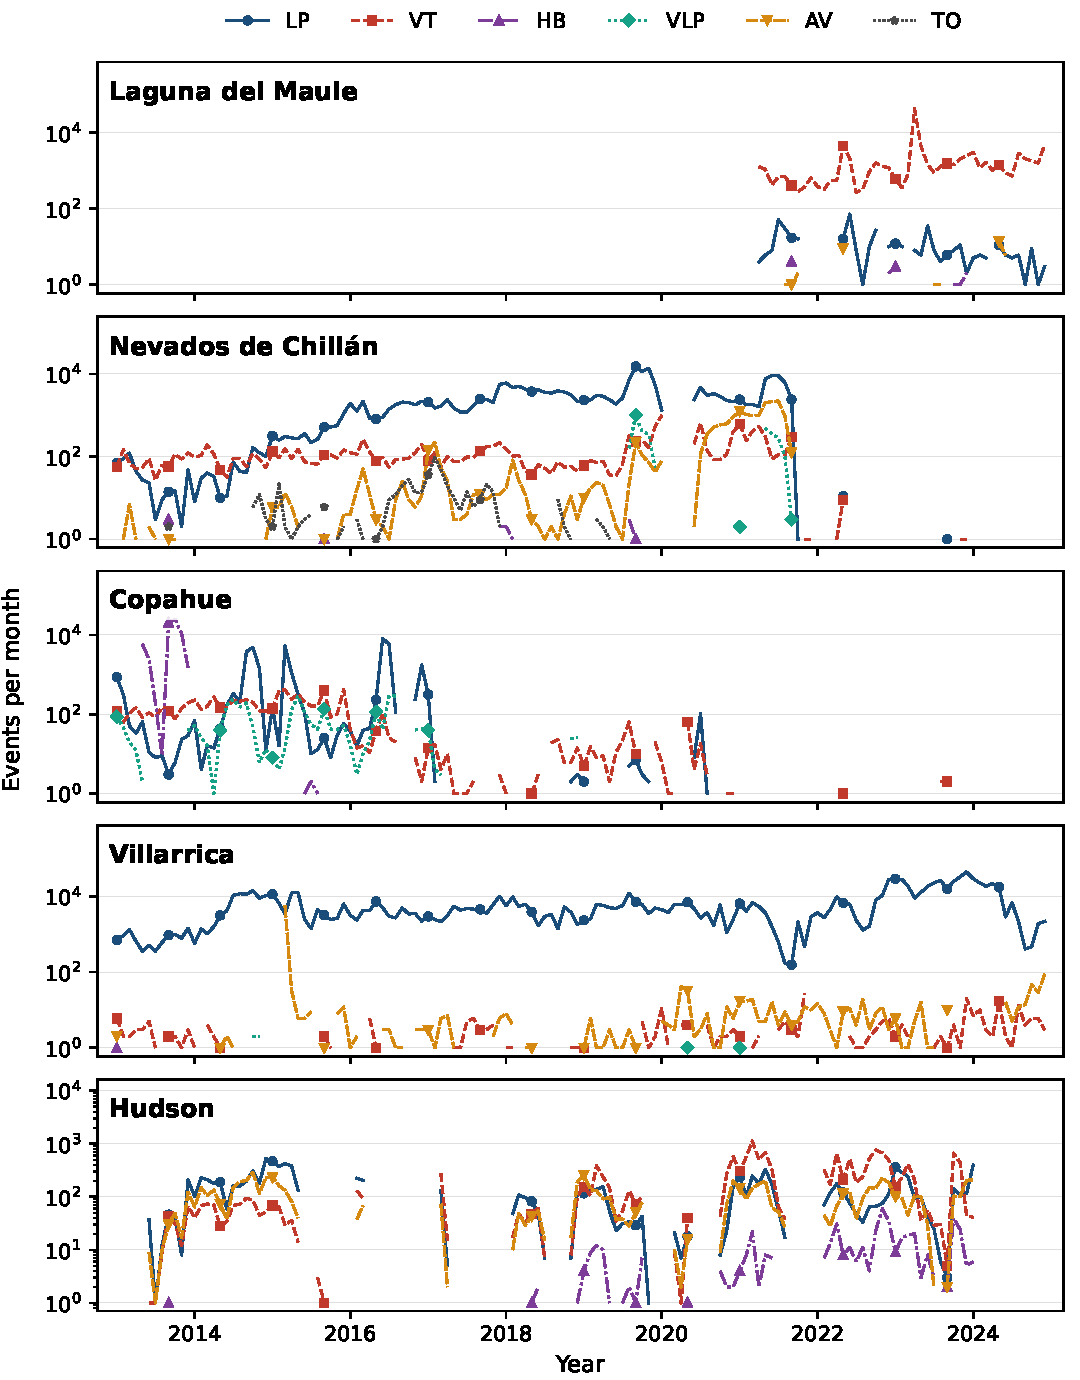
\includegraphics[width=0.91\textwidth]{fig_timeseries.pdf}
\caption{Monthly event rates for the six retained seismic classes at Laguna del
Maule, Nevados de Chill\'an, Copahue, Villarrica, and Hudson. The vertical axis
shows events per month on a logarithmic scale. Lines and symbols distinguish the
seismic classes. The analyzed interval spans April 2021--December 2024 at Laguna
del Maule, March 2013--January 2024 at Hudson, January 2013--August 2024 at
Copahue, and January 2013--December 2024 at Nevados de Chill\'an and
Villarrica (Table~\ref{tab:stations}).}
\label{fig:timeseries}
\end{figure}

Class composition also varies through time. Event rates track the temporal
development of each volcanic system, so class proportions depend on the interval
from which events are sampled (Figure~\ref{fig:timeseries}). The eruption at
Nevados de Chill\'an and the VT swarm at Laguna del Maule appear as sustained
changes in catalog composition rather than isolated rate excursions. The
temporal sampling interval therefore forms part of the statistical definition of
every training and evaluation subset.



These proportions need not follow the dominant seismicity regime alone: they
may also reflect network sensitivity, station placement, recording conditions,
and operational labeling practices. The minority classes are distributed
unevenly for the same reason. Outside Copahue and Hudson, HB support is
sparse, with only isolated populations at Villarrica, Nevados de Chill\'an,
and Laguna del Maule. TO is represented only at Nevados de Chill\'an within
the analyzed population. VLP representation is concentrated at Nevados de
Chill\'an and Copahue, with 23 events at Villarrica; Laguna del Maule and
Hudson contain no VLP events. Because the selected stations differ in
source--station distance, instrument configuration, installation date, and
background-noise level, measured classification performance may reflect
system-specific recording quality as much as source separability; the results
therefore report event-level signal-to-noise ratios alongside classification
performance.

The AV label is operationally associated with signals attributed to unstable
slopes, glacier-related mass movement, or active crater-rim processes. Hudson contains the largest relative AV population, with AV representing 22.5\%
of analyzed events, consistent with the range of surface and mass-movement
processes expected on a heavily glaciated edifice. Nevados de Chill\'an contains the second-largest relative AV population
at 6.1\%. Villarrica contributes 6{,}440 AV events in absolute terms, while its
much larger LP population limits the AV fraction to 0.7\%. AV has limited
representation at Copahue and Laguna del Maule. Volcano-class combinations
containing fewer than 100 events are excluded from training and evaluation
according to the class-support criterion defined in
Section~\ref{subsec:classsupport}. Eighteen of the thirty volcano-class
combinations of Table~\ref{tab:counts} clear that threshold: five at Nevados
de Chill\'an, four at Copahue and Hudson, three at Villarrica and two at
Laguna del Maule. Every system therefore contributes at least two classes,
and no class is admitted at every system.


\subsection{External catalogs}\label{subsec:external}

Four catalogs compiled by other agencies provide labeled records on which the
pipeline of Section~\ref{sec:methods} is applied without any parameter being
re-fitted. They serve as an external validation of the descriptors and are
not part of the analyzed population of Table~\ref{tab:counts}. This external
validation is the second stage of the programme opened in
\cite{morales_recurrence_2026}, which established the recurrence and spectral
descriptors on the five OVDAS systems alone; here the same descriptors are
measured on records the pipeline was never built from, labeled under other
operational practices. Table~\ref{tab:external} summarizes the four catalogs.

The Deception Island dataset \cite{cortes_standardization_2019} comprises two
independent deployments on the same Antarctic volcano, in 1995 and 2009, with
different stations and instruments. Records are sampled at 50~Hz. Its label
file delimits every event by a start and an end, and every LP and VT segment
of both deployments enters the review of Section~\ref{subsec:manualcut}. A
single record holds several labeled segments, typical of the swarms the
volcano produces, and each segment is reviewed as its own event.

VCSEIS \cite{zhong_deep-learning-based_2024}, distributed in SeisBench format
\cite{woollam_seisbench_2022}, covers four volcanic regions catalogued by the
Alaska Volcano Observatory, the Hawaiian Volcano Observatory, the Northern
California Earthquake Data Center and the Pacific Northwest Seismic Network
(Cascade Range). Records are sampled at 100~Hz, and each trace carries P and S
arrival samples. Class labels are taken from the catalog field that
distinguishes long-period from local events; traces carrying any other code
are left out. A random draw of 500 traces per region and class enters the
review. VCSEIS distributes one trace per station, so an earthquake recorded
at several stations appears several times in the draw; one trace per
earthquake is retained (Section~\ref{subsec:manualcut}).

The VOISS-Net training set \cite{fee_generalized_2025} labels 120~s windows
of continuous data from volcanoes in Alaska and Hawai`i, one label per window
and per network. Its Earthquake and Long Period labels enter this study as VT
and LP. The two classes come from different volcanoes: Earthquake from
K\={\i}lauea, Redoubt and Tanaga, Long Period from Veniaminof, Semisopochnoi
and Pavlof, so each of these six systems contributes a single class.
Waveforms are retrieved from the EarthScope data center at the vertical
channel of one reference station per volcano, sampled at 40, 50 or 100~Hz
depending on the station, with 60~s before and 120~s after each labeled
window. Windows are reviewed in random order within each volcano and class.

The Servicio Geol\'ogico Colombiano (SGC) provided 500 events per class from
Nevado del Ruiz, labeled LP, VT and HB by its analysts and extracted from the
waveform archive as one file per event holding the whole network, sampled at
100~Hz. The files carry no catalog onset or duration. Following the SGC, the
reference station is Olleta, with Bis as its backup; the two stations differ
in their records of the same classes, and each is treated as a separate
system (Section~\ref{subsec:manualcut}).

Across the four catalogs, the comparison is restricted to the classes they
share with the OVDAS taxonomy: LP and VT in all four, and HB at Nevado del
Ruiz. Labels for tremor, explosions, noise, regional events and other codes
have no counterpart in the OVDAS taxonomy and are left out. Each region of
VCSEIS, each volcano of VOISS-Net and each station at Nevado del Ruiz is a
separate system, in the same way as the five OVDAS systems.

\begin{table}[h]
\caption{External catalogs used for validation: the systems each contributes,
the classes it labels that match the OVDAS taxonomy, its sampling rate, and
the reference times it supplies. All records are brought to 100~Hz before
conditioning. The onset, the end of the coda and the noise window of every
event are set by the manual review of Section~\ref{subsec:manualcut}.}
\label{tab:external}
\begin{tabular}{@{}lp{3.2cm}llp{2.2cm}@{}}
\toprule
Catalog & Systems & Classes & Rate (Hz) & Reference supplied \\
\midrule
Deception Island \cite{cortes_standardization_2019} & 1 (two deployments) & LP, VT & 50 & segment start and end \\
VCSEIS \cite{zhong_deep-learning-based_2024} & Alaska, Cascade Range, Hawai`i, N. California & LP, VT & 100 & P and S arrivals \\
VOISS-Net \cite{fee_generalized_2025} & K\={\i}lauea, Redoubt, Tanaga & VT & 40--100 & 120~s labeled window \\
 & Veniaminof, Semisopochnoi, Pavlof & LP & 40--100 & 120~s labeled window \\
SGC, Nevado del Ruiz & Olleta, Bis & LP, VT, HB & 100 & none \\
\botrule
\end{tabular}
\end{table}


%%===========================================================================%%
\section{Methodology}\label{sec:methods}

This section defines the pipeline that converts a catalog entry surviving the
criteria of Section~\ref{subsec:composition} into the descriptors and the
working subsample used elsewhere in the paper, in the order in which the steps
are applied. Section~\ref{subsec:stationselection} states the criterion by
which a single station is selected at each volcanic system, fixing the
interval available for analysis. Section~\ref{subsec:conditioning} defines the fixed-length analysis
window and the conditioning applied to it, together with the criterion by
which an event is retained in the analyzed population of
Table~\ref{tab:counts}. Section~\ref{subsec:codawindow} defines the
coda-length window computed alongside it for every event, and
Section~\ref{subsec:manualcut} sets the onset, the end of the coda and the
noise window of the external records of Section~\ref{subsec:external}. Section~\ref{subsec:classsupport} states the minimum
per-volcano, per-class support required for a class to enter training and
evaluation. Section~\ref{subsec:features} computes, for every retained event,
the thirteen time-domain recurrence descriptors and the three spectral
descriptors used throughout the study. Because the steps that compare events
pairwise are quadratic in their number and therefore infeasible on the full
analyzed population, Section~\ref{subsec:sampling} draws a single
reproducible working subsample of it. This section names every variable the
pipeline fixes in advance; Section~\ref{subsec:configuration} reports the
value adopted for each.

\subsection{Station selection}\label{subsec:stationselection}

At each volcanic system, the analysis draws on a single station: the one
that combines the largest number of catalogued detections with
uninterrupted operation. Restricting the analysis to one station per system
avoids mixing records with different instrument responses and
source--station distances within a single class, at the cost of leaving
other stations of the same local network unused. This choice also fixes the
interval available for analysis, since the analyzed interval of a system is
the span over which its selected station appears as the detecting station in
the catalog, narrower than the nominal 2013--2024 request at three of the
five systems (Table~\ref{tab:stations}, Section~\ref{subsec:area}).

\subsection{Signal conditioning}\label{subsec:conditioning}

Every retained event is represented by a single fixed-length window,
beginning at the analyst-assigned onset, at the sampling rate common to all
five stations (Table~\ref{tab:stations}). The window opens at the onset so
that every sample entering a descriptor belongs to the event. An earlier
form of this window opened before the onset, and that leading segment,
being near-constant once z-scored, placed its samples within $\varepsilon$
of one another and saturated a block of the recurrence plot with spurious
recurrence. The window instead opens at the onset, avoiding this effect
entirely. The window is extracted from a longer padded segment that
extends symmetrically before the onset and beyond the end of the retained
window, which is detrended (linear) and band-pass filtered (zero-phase
Butterworth) before being trimmed to its final length. The padding at each
end holds the filter's edge transient clear of the retained window, whose
samples settle close to the values a much longer segment would yield.

Because the catalog carries no multi-station origin time
(Section~\ref{subsec:catalog}), the padded segment must come from a single,
gap-free trace at the selected station spanning the full padded interval. An
event whose station record leaves this interval incomplete, through a data
gap, an interruption, or a date before the station was installed, is excluded
at this step; together with the station restriction of
Section~\ref{subsec:composition}, this is what separates the six-class
totals of Table~\ref{tab:rawcounts} from the analyzed population of
Table~\ref{tab:counts}. A second, far rarer exclusion applies after
filtering: an event whose filtered window has zero variance has no defined
z-score and is excluded as well.

A signal-to-noise ratio is computed from the same padded segment, over a
short noise window preceding the onset and the signal window. It is
reported alongside classification results, where it distinguishes a class
that is easier to recognize because of where it is recorded from one that is
easier to recognize because its source is distinctive:
\begin{equation}
\mathrm{SNR_{dB}} = 20\log_{10}\frac{\mathrm{RMS}(\text{signal window})}{\mathrm{RMS}(\text{noise window})}.
\end{equation}
Both windows entering this ratio are measured on the segment band-passed to
a band narrower than the analysis band. Below its lower edge the
record at these stations is dominated by the secondary oceanic microseism,
whose amplitude follows ocean swell and station distance to the coast, and
which the analysis band admits by design because VLP events radiate there.
Measuring the ratio over the narrower band keeps it a statement about recording
quality in the band where the events of Table~\ref{tab:counts} radiate. VLP events, whose
energy extends below this band, are the one class the ratio understates.
The signal window is z-scored (zero mean, unit variance) before any
descriptor is computed from it, so that the descriptors of
Section~\ref{subsec:features} are computed on a dimensionless signal. Any
duration reported elsewhere in this paper is the analyst-assigned duration of
Section~\ref{subsec:catalog}. Figure~\ref{fig:window} sets out the intervals
this section defines; Section~\ref{subsec:configuration} reports every duration,
offset, and band named above.

\begin{figure}[H]
\centering
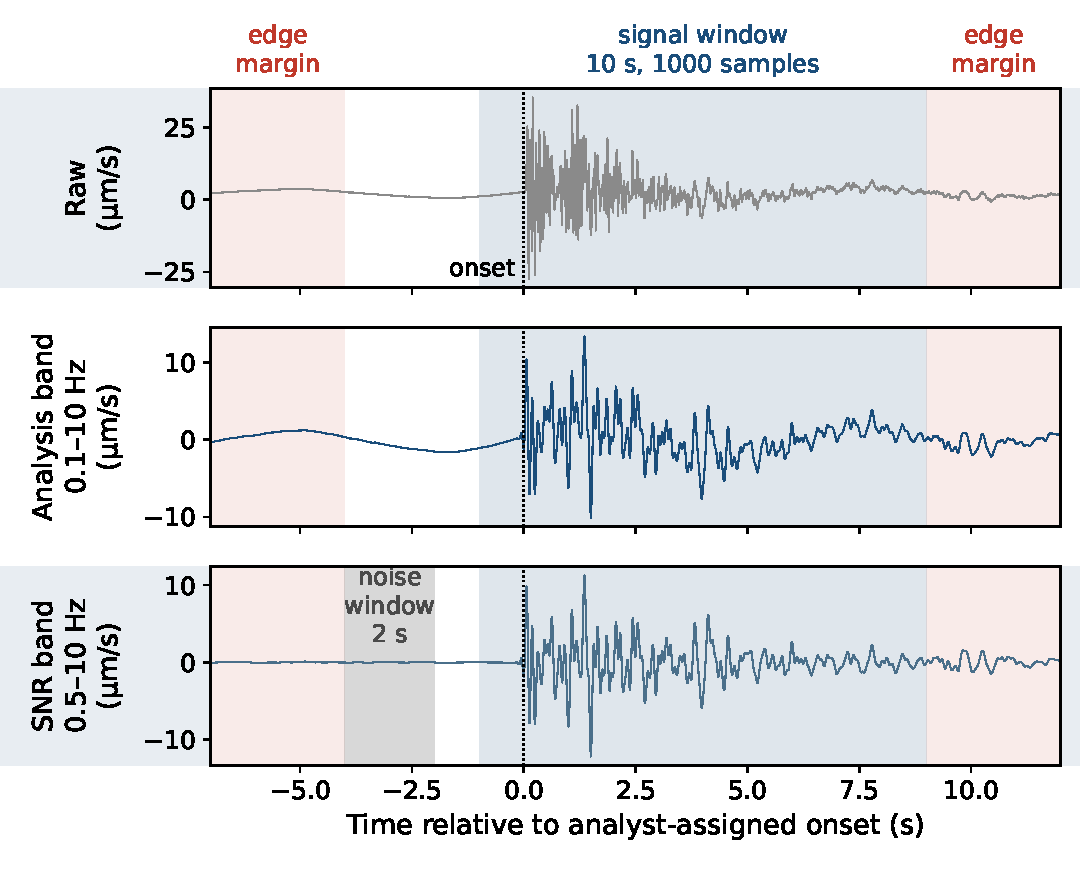
\includegraphics[width=0.94\textwidth]{fig_window.pdf}
\caption{Extraction and conditioning of the analysis window, drawn to scale
against the analyst-assigned onset (dotted line), with the signal-to-noise
ratio of the example event reported on the panel. The example is a VT event
recorded at Hudson on station HUDZ.
Amplitudes are ground velocity, obtained from the recorded counts by the
station's sensitivity, which is flat across the band shown. Top: the raw
padded segment. Bottom: the same segment after linear detrending and the
zero-phase band-pass to the analysis band, applied to the segment as a whole;
this is also the band over which the signal-to-noise ratio is measured, so a
single conditioned segment carries both. Shading
marks the intervals the conditioning defines: the edge margins at each
end, which absorb the filter's edge transient and are discarded; the
noise window, marked on the panel where it is
measured; and the signal window, the
record every descriptor of Section~\ref{subsec:features} is computed from.
Durations, offsets, and bands are reported in Section~\ref{subsec:configuration}. The
separation between the noise window and the onset
keeps an emergent arrival out of the noise measurement.}
\label{fig:window}
\end{figure}

\subsection{Coda-length window}\label{subsec:codawindow}

A second window represents every event alongside the fixed-length window of
Section~\ref{subsec:conditioning}. It opens at the same onset and closes at
the end of the coda, so its length follows the duration of the event. The
two windows answer different questions: the fixed-length window compares
events over an identical interval, dominated by the onset and the early coda,
while the coda-length window describes each event as a whole. Computing the
sixteen descriptors of Section~\ref{subsec:features} on both, for the same
events, shows which properties of a class are carried by its onset and which
by its full coda.

At the OVDAS systems the end of the coda is the analyst-assigned duration of
Section~\ref{subsec:catalog}; at the external catalogs it is the end set in
the manual review of Section~\ref{subsec:manualcut}. The coda-length window
is extracted from a padded segment in the same way as the fixed-length one,
with a noise window and a separation before the onset and an edge margin
after the end of the coda, and is band-passed to its own analysis band before
being trimmed. Events shorter than a minimum duration hold too few samples
for the recurrence descriptors and are excluded from this window, and the
window is capped at a maximum length, over which the descriptors of a long
coda are measured on its first part.
Section~\ref{subsec:configuration} reports the band, the noise window, the
margins and both limits.

\subsection{Manual segmentation of the external records}\label{subsec:manualcut}

The external catalogs supply labels but not the three references the windows
require, an onset, the end of the coda and a pre-event noise window, in a
form comparable to the OVDAS catalog (Table~\ref{tab:external}). The three
are therefore set by hand for every external event, by a single analyst,
following one protocol across the four catalogs. Each record is displayed as
its band-passed trace and its spectrogram, together with the reference the
catalog supplies: the labeled segment at Deception Island, the P and S
arrivals in VCSEIS, the 120~s labeled window in VOISS-Net. The analyst marks
the onset at the first arrival of the labeled event, the end of the coda
where the signal returns to the pre-event level, and a noise window
immediately before the onset, free of other events where the record allows
it.

An event is retained when its onset falls within the reference the catalog
supplies and its coda can be delimited within the record. It is discarded
when no event is visible within that reference, when it lasts less than the
minimum duration of Section~\ref{subsec:codawindow}, or when the record does
not hold the padded segment of either window. At Nevado del Ruiz, an event
not visible at Olleta is reviewed at Bis, and the station on which it is cut
is recorded with the event. The analyst may also revise a label; an event
relabeled as a tornillo (TO) is kept within LP, the class it was catalogued
as, and flagged.

An event that enters the review more than once is retained once: an
earthquake recorded at several VCSEIS stations, identified by its catalog
source identifier, and an event spanning two consecutive VOISS-Net windows or
two consecutive SGC files, identified by onsets less than 3~s apart at the
same system. Of each group, the copy whose onset falls within its labeled
reference and has the highest signal-to-noise ratio is retained.

All external records are brought to 100~Hz before the conditioning of
Section~\ref{subsec:conditioning}, so that the embedding of
Section~\ref{subsec:features}, defined in samples, spans the same time at
every system. From that point on, both windows and all sixteen descriptors
are computed with the same code and parameters as at the OVDAS systems.


\subsection{Class support criterion}\label{subsec:classsupport}

A class is included in training and evaluation at a given volcanic system
only if that volcano-class combination reaches a minimum event count in the
analyzed population of Table~\ref{tab:counts}; Section~\ref{subsec:configuration}
states that threshold. A combination below this
threshold is excluded from that system's experiments, while its events
remain part of the analyzed population reported elsewhere in this paper
(Table~\ref{tab:counts}, Figure~\ref{fig:timeseries}). The threshold marks
the point from which a class carries enough events to represent the range it
spans at that system, which is what both feature extraction and
classification draw on, and from which a measured performance reflects a
stable property of the class rather than the particular events that entered
the sample. The two isolated cases of Section~\ref{subsec:composition}, one
HB event at Villarrica and one AV event at Copahue, fall far below it.

The criterion is evaluated on the analyzed population, but the experiments
run on the working subsample drawn in Section~\ref{subsec:sampling}. The two are reconciled there: a class admitted
by this criterion receives a floor quota in the subsample, so that clearing
the threshold in Table~\ref{tab:counts} also guarantees usable support in the
set the classifier is actually trained and scored on.

The threshold is a convention fixed in advance and applied uniformly to every
volcano-class combination in the study. Holding it constant keeps the set of
classes a system contributes independent of the results later obtained from
them, and Section~\ref{subsec:configuration} reports which combinations it admits at
each system.

\subsection{RQA and spectral feature extraction}\label{subsec:features}

Sixteen descriptors are computed for every event retained by
Section~\ref{subsec:conditioning}: thirteen time-domain recurrence
descriptors and three spectral descriptors. Both act on the same z-scored
signal window; no descriptor combines information from more than one event.

The thirteen recurrence descriptors: $DET$, $L$, $L_{max}$, $DIV$, $L_{entr}$, $LAM$, $TT$,
$V_{max}$, $V_{entr}$, $W$, $W_{max}$, $W_{div}$, and $W_{entr}$, are computed by recurrence
quantification analysis (RQA) \cite{marwan_recurrence_2007} on the z-scored window, with a fixed
embedding dimension, time delay, and Theiler correction (immediate temporal
neighbors excluded from the neighborhood count); Section~\ref{subsec:configuration}
reports the value adopted for each.
Diagonal, vertical, and white vertical line structures are counted from a
fixed minimum line length, reported in Section~\ref{subsec:configuration}
(Figure~\ref{fig:rqa}). The neighborhood radius $\varepsilon$ is
selected per event, not fixed in advance: the smallest radius in a candidate
grid whose recurrence rate ($RR$) falls within a target band is
accepted; if no radius in the grid meets this criterion, the radius whose $RR$
is closest to the midpoint of a narrower fallback band
is used instead. Section~\ref{subsec:extractionvalues} reports the radius adopted
at each system, and Section~\ref{subsec:configuration} reports the radius grid and both
bands. $DIV$ and $W_{div}$, both defined as the reciprocal of a
longest-line length, are set to missing rather than infinite when that
length is zero; if every radius in the grid fails to produce a usable
recurrence plot, all thirteen descriptors, together with $\varepsilon$ and
RR, are left missing for that event. Frequency information enters through the
three spectral scalars defined next.

The three spectral descriptors, $f_{\text{peak}}$, $SR$, and $FI$, are
computed from the real FFT of the filtered (non-z-scored) signal window.
$f_{\text{peak}}$ and $SR$ are evaluated over a band narrower than the full
filter passband, because the zero-phase Butterworth filter of
Section~\ref{subsec:conditioning} is not flat approaching its upper corner;
Section~\ref{subsec:configuration} reports the evaluation band and the filter's
amplitude response at representative frequencies within it. Restricting the
evaluation band to the flat part of
the response keeps these descriptors from reflecting the filter rather than
the signal. $f_{\text{peak}}$ is the frequency of maximum spectral amplitude
in that band, and $SR$ is the ratio of mean to maximum spectral amplitude over
the same band, following \cite{cui_subdivision_2021}, a measure of spectral
concentration, low when energy is confined to a narrow band and approaching
1 for a flat, broadband spectrum. $FI$ contrasts two narrower bands separated
by a gap rather than a single cutoff, following \cite{cui_subdivision_2021} and
\cite{buurman_seismic_2010}:
\begin{equation}
\mathrm{FI} = \log_{10}\frac{\overline{A}(\text{high band})}{\overline{A}(\text{low band})},
\end{equation}
where $\overline{A}$ denotes mean spectral amplitude over the stated band and
Section~\ref{subsec:configuration} reports the two bands.

The VLP class sits outside the range these three descriptors resolve. A very
long period event radiates, by the definition that separates the class from
LP, at frequencies lower than the classes it is contrasted against, and its
dominant frequency lies below the evaluation band. For a VLP event
$f_{\text{peak}}$ therefore reports the strongest spectral component the band
admits, and the class characteristic that most directly distinguishes it, the
frequency at which it radiates most energy, is a quantity this measurement
places a lower bound on. The three descriptors stay comparable across events,
since one band applies to all of them; the reading of
$f_{\text{peak}}$ as a physical dominant frequency holds for the other five
classes. Section~\ref{subsec:extractionvalues} reports how often a VLP event peaks at
the lower edge of the band.
Figure~\ref{fig:spectral} shows the three descriptors measured on one event
of each class.

\begin{figure}[H]
\centering
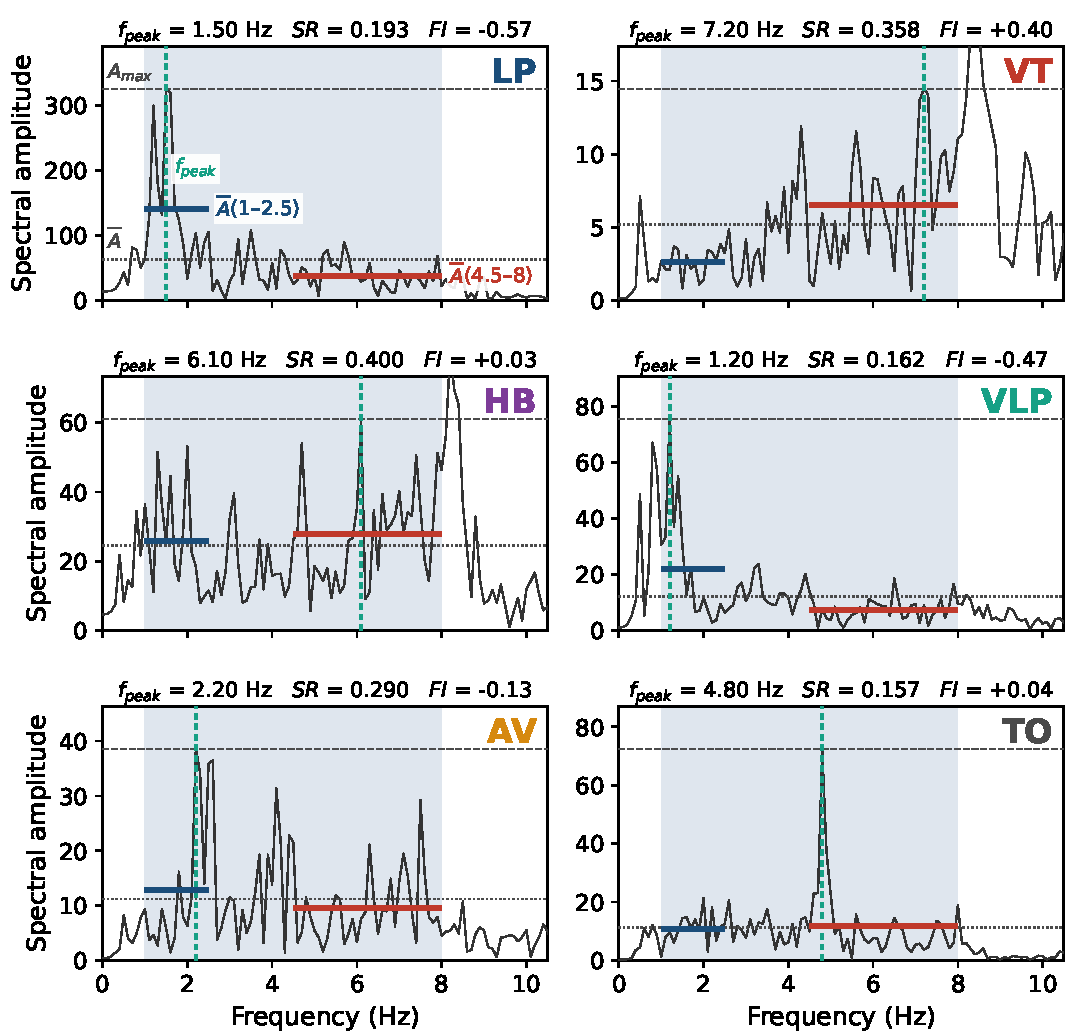
\includegraphics[width=0.98\textwidth]{fig_spectral.pdf}
\caption{The three spectral descriptors, measured on one event of each
retained class. The six events are those of Figure~\ref{fig:gallery} and
Figure~\ref{fig:rqa}; the spectrum shown is the one the descriptors are
computed from, the FFT of the conditioned window before z-scoring, which
differs from the normalized display spectrum of Figure~\ref{fig:gallery}.
Shading marks the evaluation band reported in Section~\ref{subsec:configuration}. On
each panel the dashed and dotted horizontal lines give the maximum and mean
spectral amplitude over that band, whose ratio is $SR$, and the dashed
vertical line marks $f_{\text{peak}}$. The two coloured segments give the
mean amplitude over each of the bands entering $FI$, drawn at the height
that enters the ratio. Values appear above each panel. The labels are drawn
on the LP panel only.}
\label{fig:spectral}
\end{figure}

\begin{figure}[H]
\centering
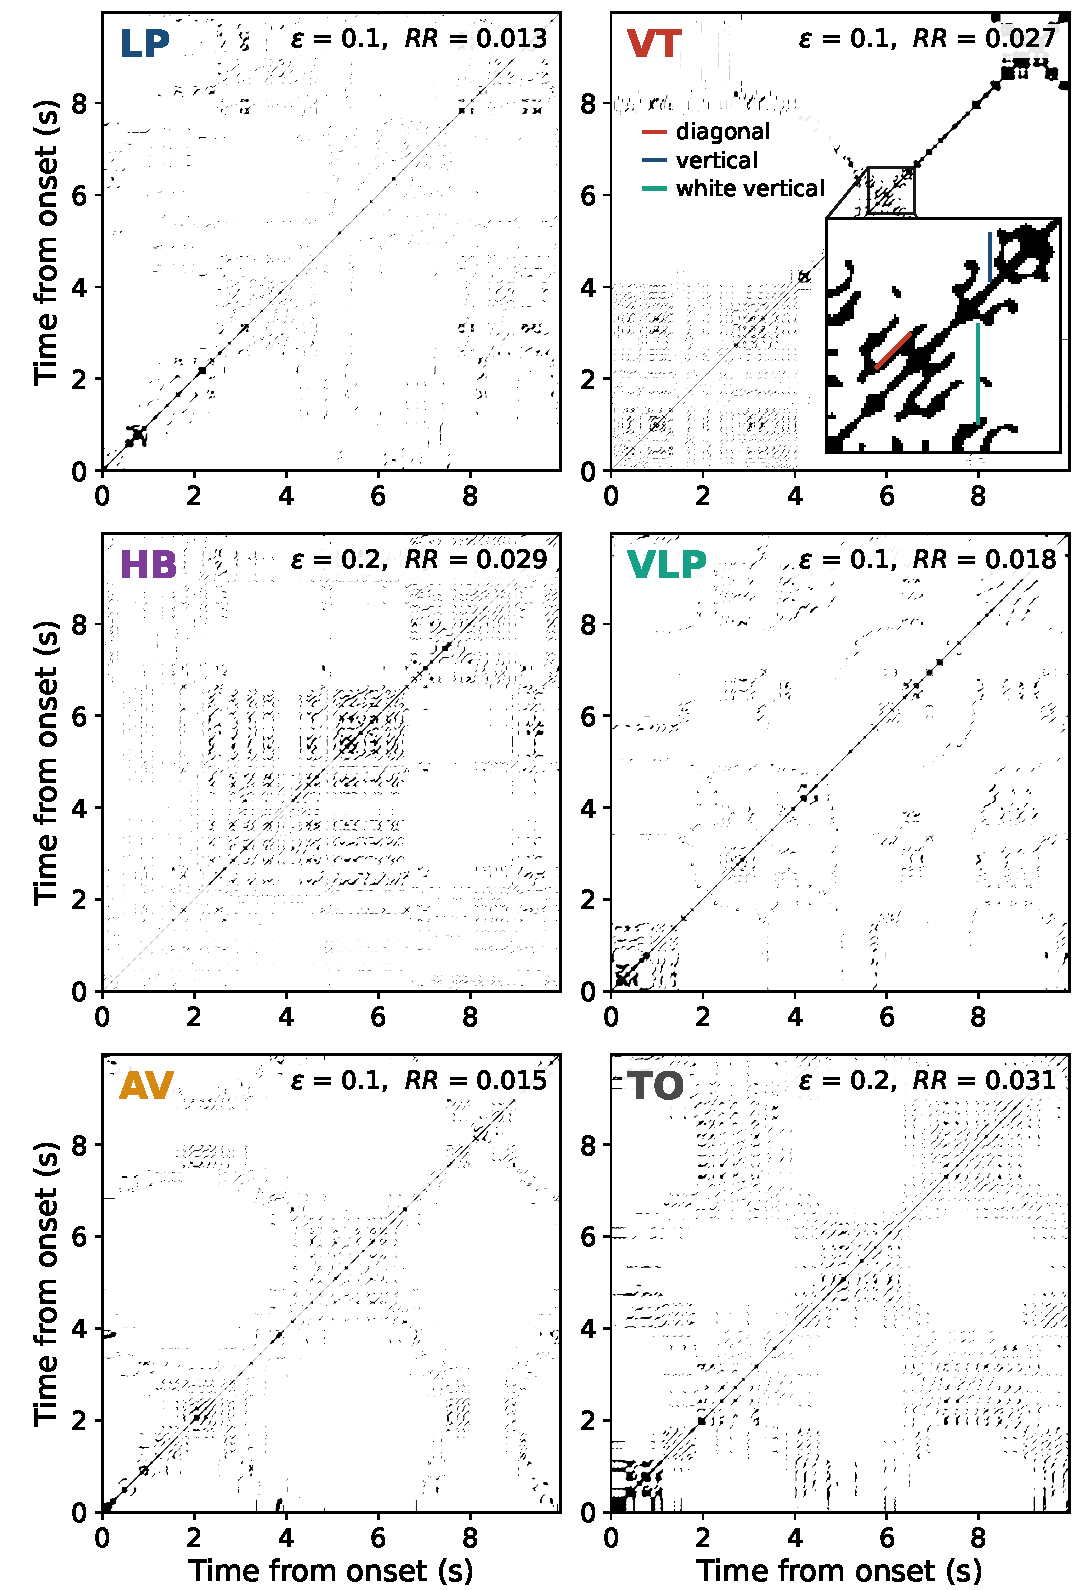
\includegraphics[width=0.68\textwidth]{fig_rqa.pdf}
\caption{Recurrence plot of one event of each retained class, computed on the
z-scored signal window at the radius $\varepsilon$ the criterion of this
section selects for that event, with the resulting recurrence rate $RR$. The
six events are those of Figure~\ref{fig:gallery}, so each plot can be read
against the waveform and spectrum shown there. Axes run from the onset, and
the line of identity is retained. The inset on the VT panel enlarges a
square taken from the middle of the window, at the scale reported in
Section~\ref{subsec:configuration}, and marks the three line
structures the thirteen descriptors quantify: diagonal lines, from which $DET$, $L$, $L_{max}$, $DIV$ and
$L_{entr}$ follow; vertical lines, giving $LAM$, $TT$, $V_{max}$ and
$V_{entr}$; and white vertical lines, giving $W$, $W_{max}$, $W_{div}$ and
$W_{entr}$. Each marked structure is the longest of its kind within the
inset, offset by a few samples so as not to cover it.}
\label{fig:rqa}
\end{figure}

\section{Results}\label{sec:results}

\section{Conclusion}\label{sec:conclusion}

\backmatter

\bmhead{Supplementary information}

\bmhead{Acknowledgements}

\section*{Declarations}
\begin{itemize}
\item Funding: Not applicable.
\item Conflict of interest/Competing interests: Not applicable.
\item Ethics approval and consent to participate: Not applicable.
\item Consent for publication: Not applicable.
\item Data availability: % TODO
\item Materials availability: Not applicable.
\item Code availability: % TODO
\item Author contribution: % TODO
\end{itemize}

\bibliography{references}

\end{document}